%%%%%%%%%%%%%%%%%%%%%%%%%%%%%%%%%%%%%%%%%
% Journal Article
% LaTeX Template
% Version 1.3 (9/9/13)
%
% This template has been downloaded from:
% http://www.LaTeXTemplates.com
%
% Original author:
% Frits Wenneker (http://www.howtotex.com)
%
% License:
% CC BY-NC-SA 3.0 (http://creativecommons.org/licenses/by-nc-sa/3.0/)
%
%%%%%%%%%%%%%%%%%%%%%%%%%%%%%%%%%%%%%%%%%

%----------------------------------------------------------------------------------------
%	PACKAGES AND OTHER DOCUMENT CONFIGURATIONS
%----------------------------------------------------------------------------------------
\documentclass[twoside]{article}

\usepackage{lipsum} % Package to generate dummy text throughout this template

\usepackage[sc]{mathpazo} % Use the Palatino font
\usepackage[T1]{fontenc} % Use 8-bit encoding that has 256 glyphs
\linespread{1.05} % Line spacing - Palatino needs more space between lines
\usepackage{microtype} % Slightly tweak font spacing for aesthetics
\usepackage{amsmath}

\usepackage[hmarginratio=1:1,top=32mm,columnsep=20pt]{geometry} % Document margins
\usepackage{multicol} % Used for the two-column layout of the document
\usepackage[hang, small,labelfont=bf,up,textfont=it,up]{caption} % Custom captions under/above floats in tables or figures
\usepackage{booktabs} % Horizontal rules in tables
\usepackage{float} % Required for tables and figures in the multi-column environment - they need to be placed in specific locations with the [H] (e.g. \begin{table}[H])
\usepackage{hyperref} % For hyperlinks in the PDF
\restylefloat{figure}
\usepackage{graphicx}

\usepackage{lettrine} % The lettrine is the first enlarged letter at the beginning of the text
\usepackage{paralist} % Used for the compactitem environment which makes bullet points with less space between them

\usepackage{abstract} % Allows abstract customization
\renewcommand{\abstractnamefont}{\normalfont\bfseries} % Set the "Abstract" text to bold
%\renewcommand{\abstracttextfont}{\normalfont\small\itshape} % Set the abstract itself to small italic text

\usepackage{titlesec} % Allows customization of titles
%\renewcommand\thesection{\Roman{section}} % Roman numerals for the sections
%\renewcommand\thesubsection{\Roman{subsection}} % Roman numerals for subsections
%\titleformat{\section}[block]{\large\scshape\centering}{\thesection.}{1em}{} % Change the look of the section titles
\titleformat{\subsection}[block]{\large}{\thesubsection.}{1em}{} % Change the look of the section titles

\usepackage{fancyhdr} % Headers and footers
\pagestyle{fancy} % All pages have headers and footers
\fancyhead{} % Blank out the default header
\fancyfoot{} % Blank out the default footer
\fancyhead[C]{Heavy Photon Search Collaboration $\bullet$ \today} % Custom header text
\fancyfoot[RO,LE]{\thepage} % Custom footer text
\usepackage{authblk}
%----------------------------------------------------------------------------------------
%	TITLE SECTION
%----------------------------------------------------------------------------------------

\title{\vspace{-15mm}\fontsize{20pt}{10pt}\selectfont\textbf{Implementation of pulse fitting cosmic signals to calibrate the HPS ECal}} % Article title
\author[1]{Luca Marsicano\thanks{luca.marsicano@ge.infn.it}}
\author[2]{Holly Szumila-Vance\thanks{hszumila@jlab.org}}
\affil[1]{Instituto Nazionale di Fisica Nucleare, Sezione di Genova, Genova, Italy}
\affil[2]{Old Dominion University, Norfolk, VA}
\renewcommand\Authands{ and }
\date{}

%----------------------------------------------------------------------------------------

\begin{document}

\maketitle % Insert title

\thispagestyle{fancy} % All pages have headers and footers

%----------------------------------------------------------------------------------------
%	ABSTRACT
%----------------------------------------------------------------------------------------

\begin{abstract}

The electromagnetic calorimeter (ECal) of the Heavy Photon Search (HPS) experiment is sensitive to measuring signals from cosmic ray muons. The use of cosmic ray muons to calibrate the ECal is critical in establishing baseline gains prior to receiving beam, calibrating edge crystals, and calibrating those crystals not in the acceptance for  elastically-scattered electrons. This note describes an improved procedure that can calibrate the ECal by pulse-fitting the raw FADC cosmic signal waveform requiring less time to collect cosmic ray signals than in previous procedures. Additionally, this note provides details on the software package needed to complete the calibration.  

\end{abstract}
%----------------------------------------------------------------------------------------
%	ARTICLE CONTENTS
%----------------------------------------------------------------------------------------

\section{Introduction}
The HPS ECal consists of 442 PbWO$_4$ scintillating crystals from the former CLAS Inner Calorimeter in Hall B at Jefferson Lab. In an upgrade, prior to HPS experimental running, the crystals were re-fitted with large area avalanche photo-diodes (10$\times$10~mm$^2$) that increased the sensitivity of the detector to smaller signals. The full detector read out is described in detail in~\cite{balossino_hps_2016}. Prior to 2016 experimental running, the signals from the ECal were split between the FADC250s and the TDCs to allow for the full commissioning of the new FADC250s. After the Engineering Run in 2015, the splitter was removed so that 100$\%$ of the signal coming from the ECal was go to the FADC250 due to their demonstrated reliability. The FADC250s were run in full waveform readout so that the signals could be examined and analyzed offline. 
\begin{figure}[hbt]
%\begin{center}
\begin{minipage}{0.45\textwidth}
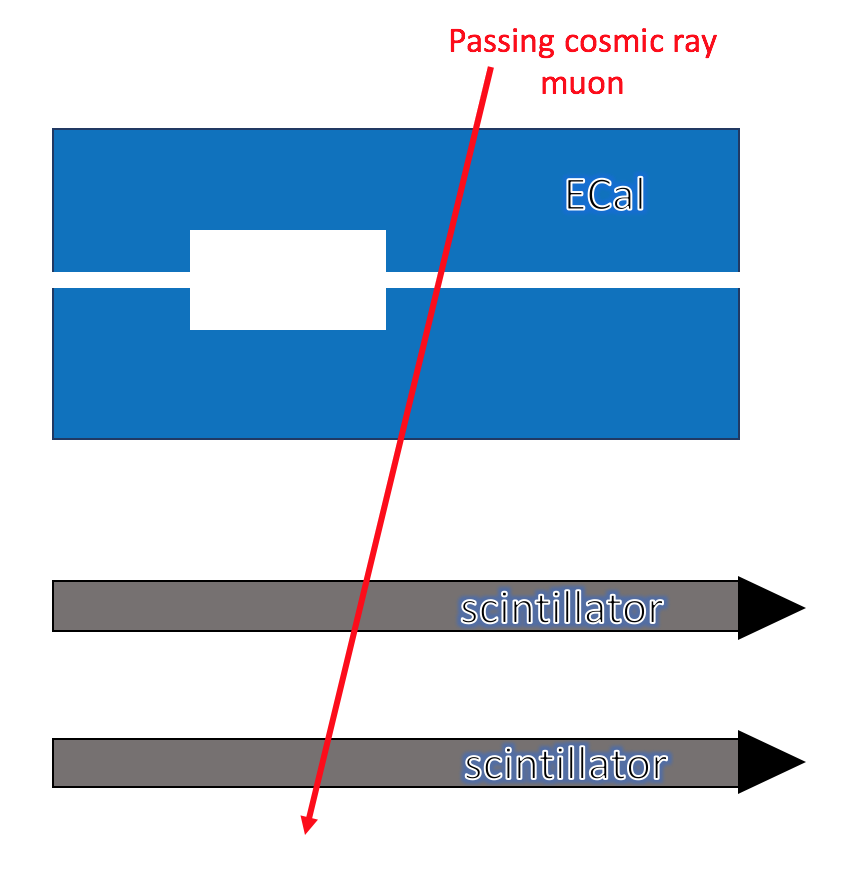
\includegraphics[width=\textwidth]{pics/cosmicSketch.png}
%\end{center}
\end{minipage}\hfill\begin{minipage}{0.45\textwidth}
 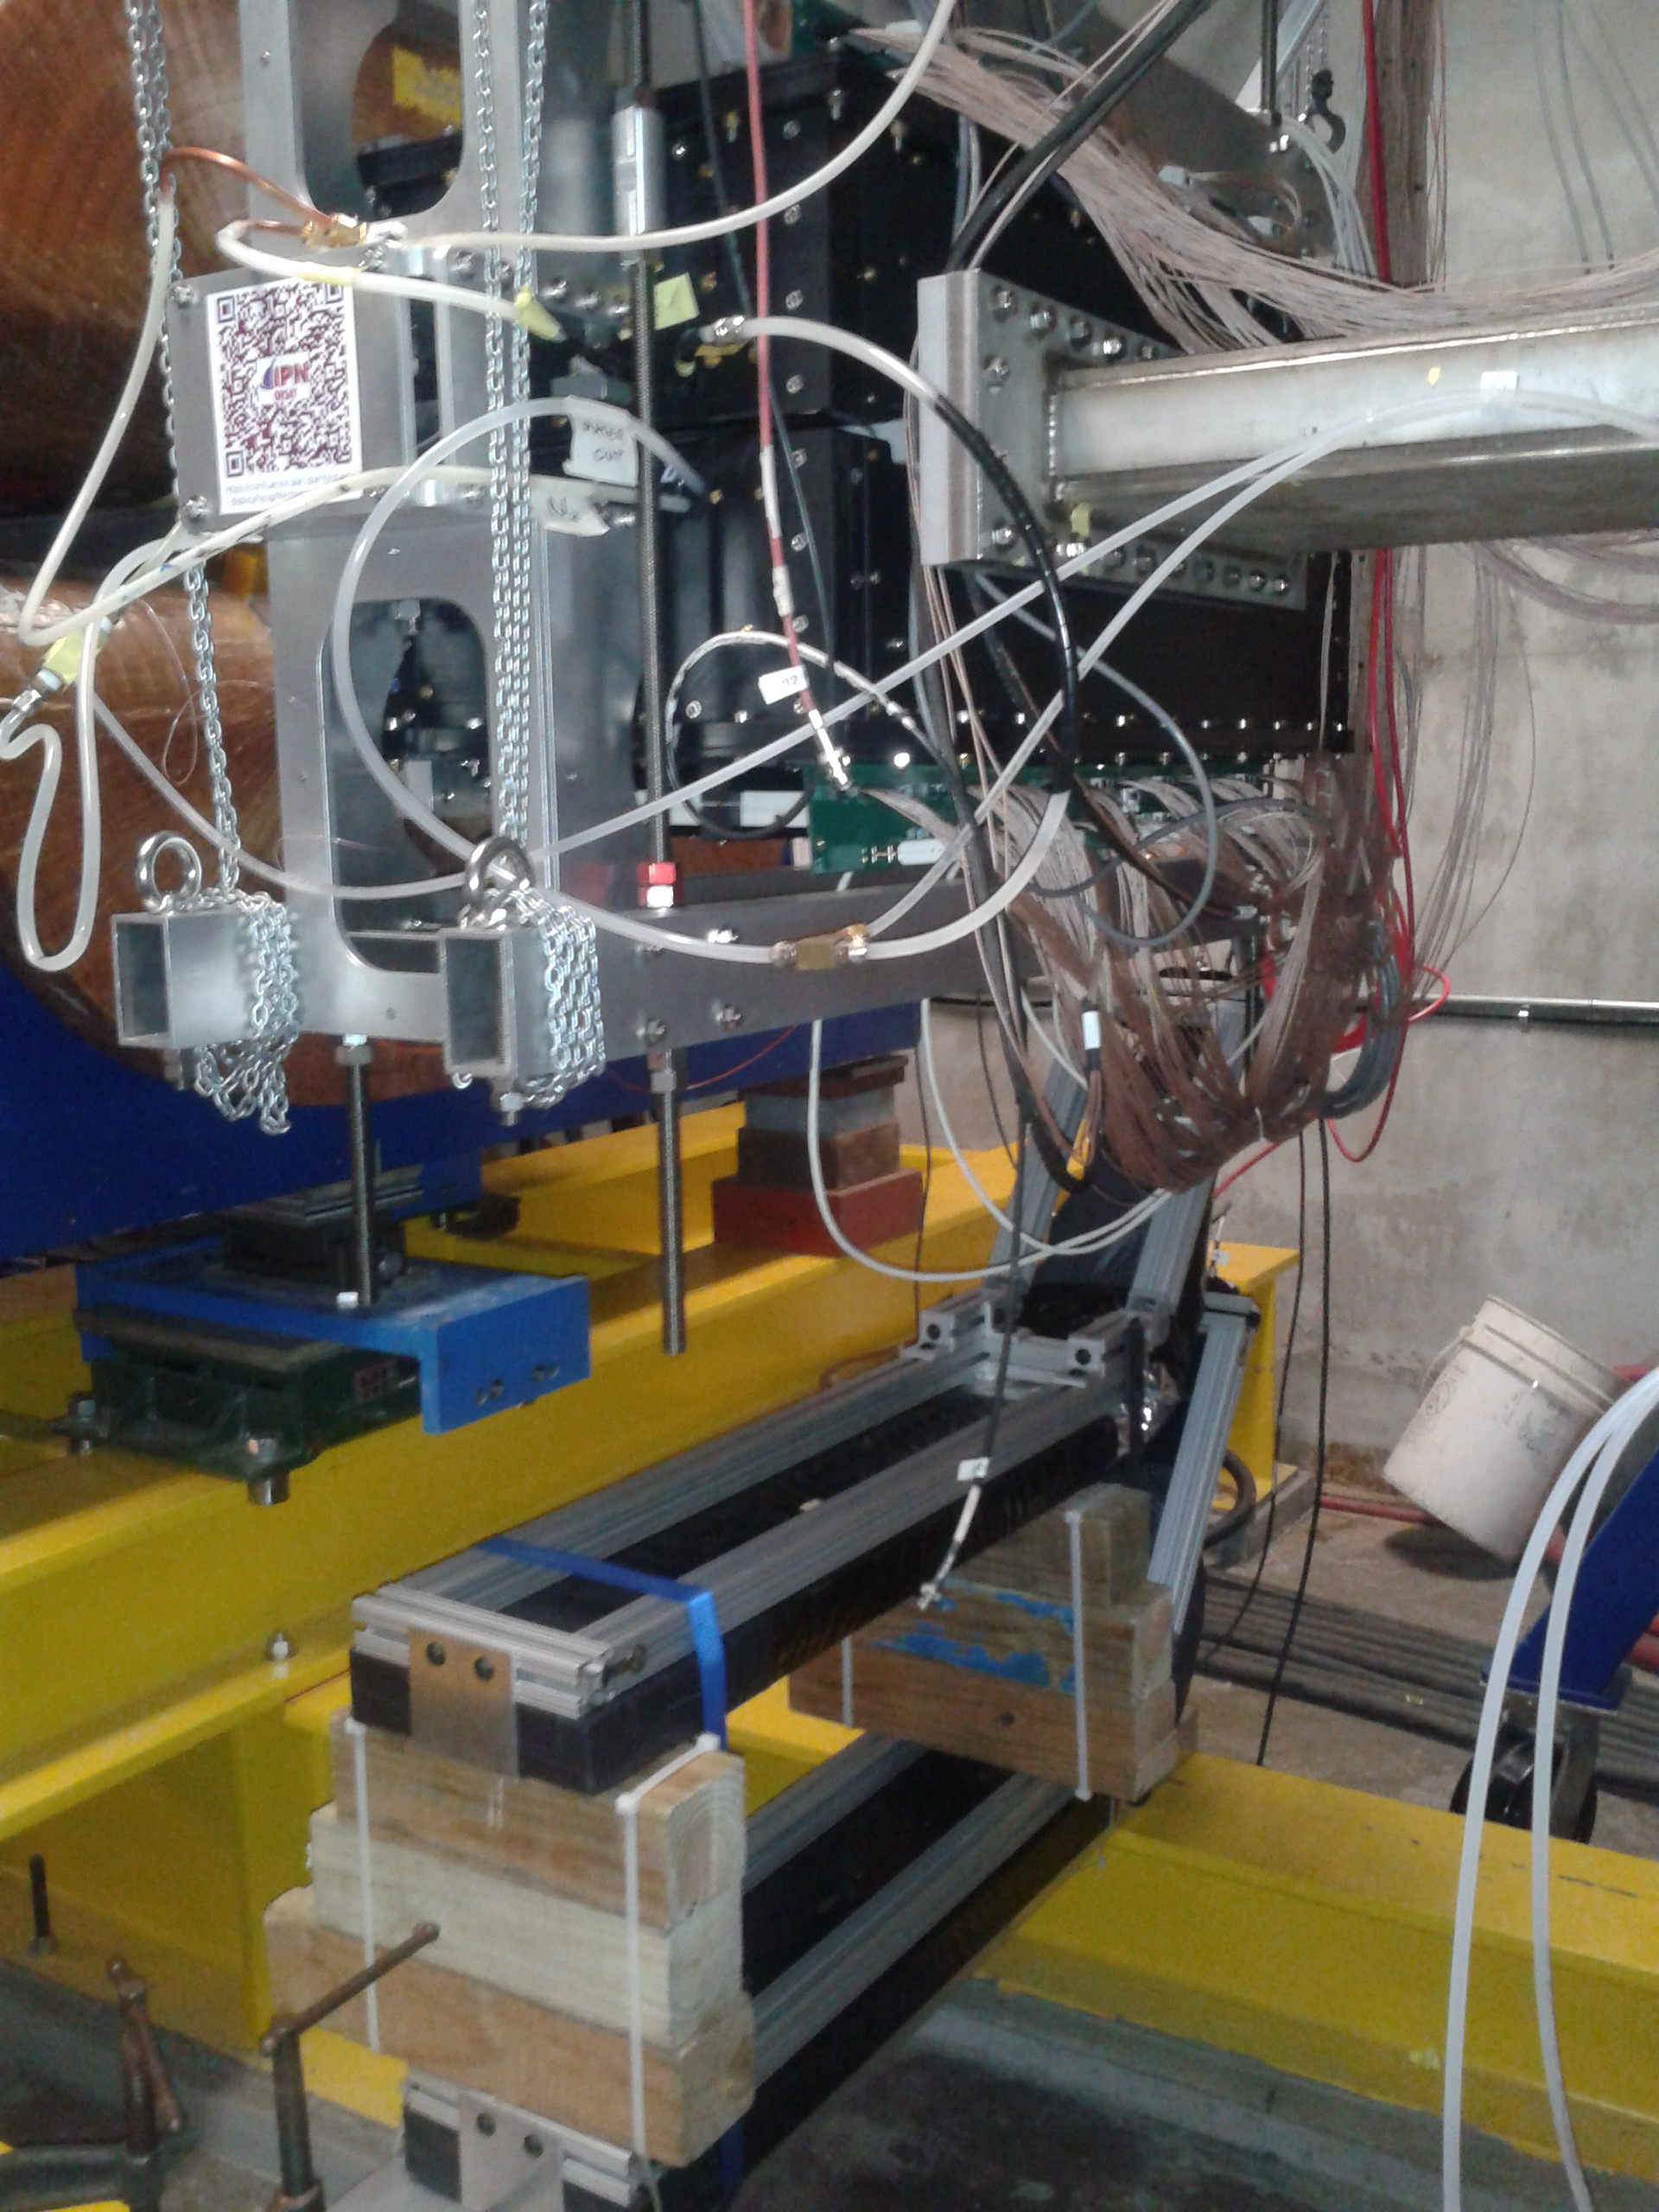
\includegraphics[width=\textwidth]{pics/cosmicPic.jpg}
 \end{minipage}
 \caption[Setup for the cosmic trigger]{A schematic showing the ECal (viewed from downstream) is shown on the left. A cosmic event is triggered when a cosmic ray muon passes vertically through the detector and is detected by both scintillators, located below. The actual installed set up is shown with a similar view from downstream on the right.}
  \label{fig:cosmicSetup}
\end{figure}
Prior to running the ECal with the electron beam, the full detector was able to calibrated using signals from passing cosmic ray muons. These signals were detectable by the ECal due to the upgraded electronics using the large area avalanche photo-diodes. The experimental setup for triggering and reading out cosmic signals in the ECal is shown in Figure~\ref{fig:cosmicSetup}.\\
\indent The previously used method of calibrating the ECal using cosmic signals is described in \cite{szumila-vance_hps_2016}. An overview is described here. After a cosmic signal is measured from the coincidence of the two triggering scintillators external to the ECal, all 442 modules were read out by the DAQ. The general trigger rate measured at the DAQ was approximately 7~Hz. Offline, a geometric selection of cuts was applied to the data to identify cosmic signals that could be used for calibration. The module of interest was first identified with a threshold crossing in the raw waveform spectra. The cuts required that no threshold crossing in the raw waveform occurred in crystals immediately adjacent in the same row. Further cuts required that adjacent crystals vertically had to have also measured a threshold crossing. If this criteria was met, then the information for that crystal was kept for the calibration.\\
\indent The calibration procedure selected a window prior to the signal window in the raw FADC wave spectrum to calculate an average event-by-event pedestal for a particular channel. The integral was extracted by summing the raw waveform spectrum in the signal window and subtracting the corresponding pedestal. This pulse-integral was recorded over many events and fit with a Landau-Gaussian convolution. The peak of the fit was obtained numerically and corresponded to the FADC calibration point. The procedure described above will differ from that described by this note. The acquisition of the data will be the same, but the cuts and fits to extract the gain for each module will be different and described in detail. 

%------------------------------------------------
\section{Method}
The calibration procedure that follows was tuned and developed on the cosmic ray data obtained after the removal of the splitters from the readout chain in 2016. The signal amplitudes in the raw FADC waveform were visually larger than those seen when taken with the splitters. Some time was spent in determining an adequate threshold for a clear minimum ionization peak in the data and keeping good events. With minimal cuts, a cosmic ray passing vertically through the ECal produces some signal in all ten layers as shown in Figure~\ref{rawColumn}.\\
\begin{figure}[htb]
  \centering
      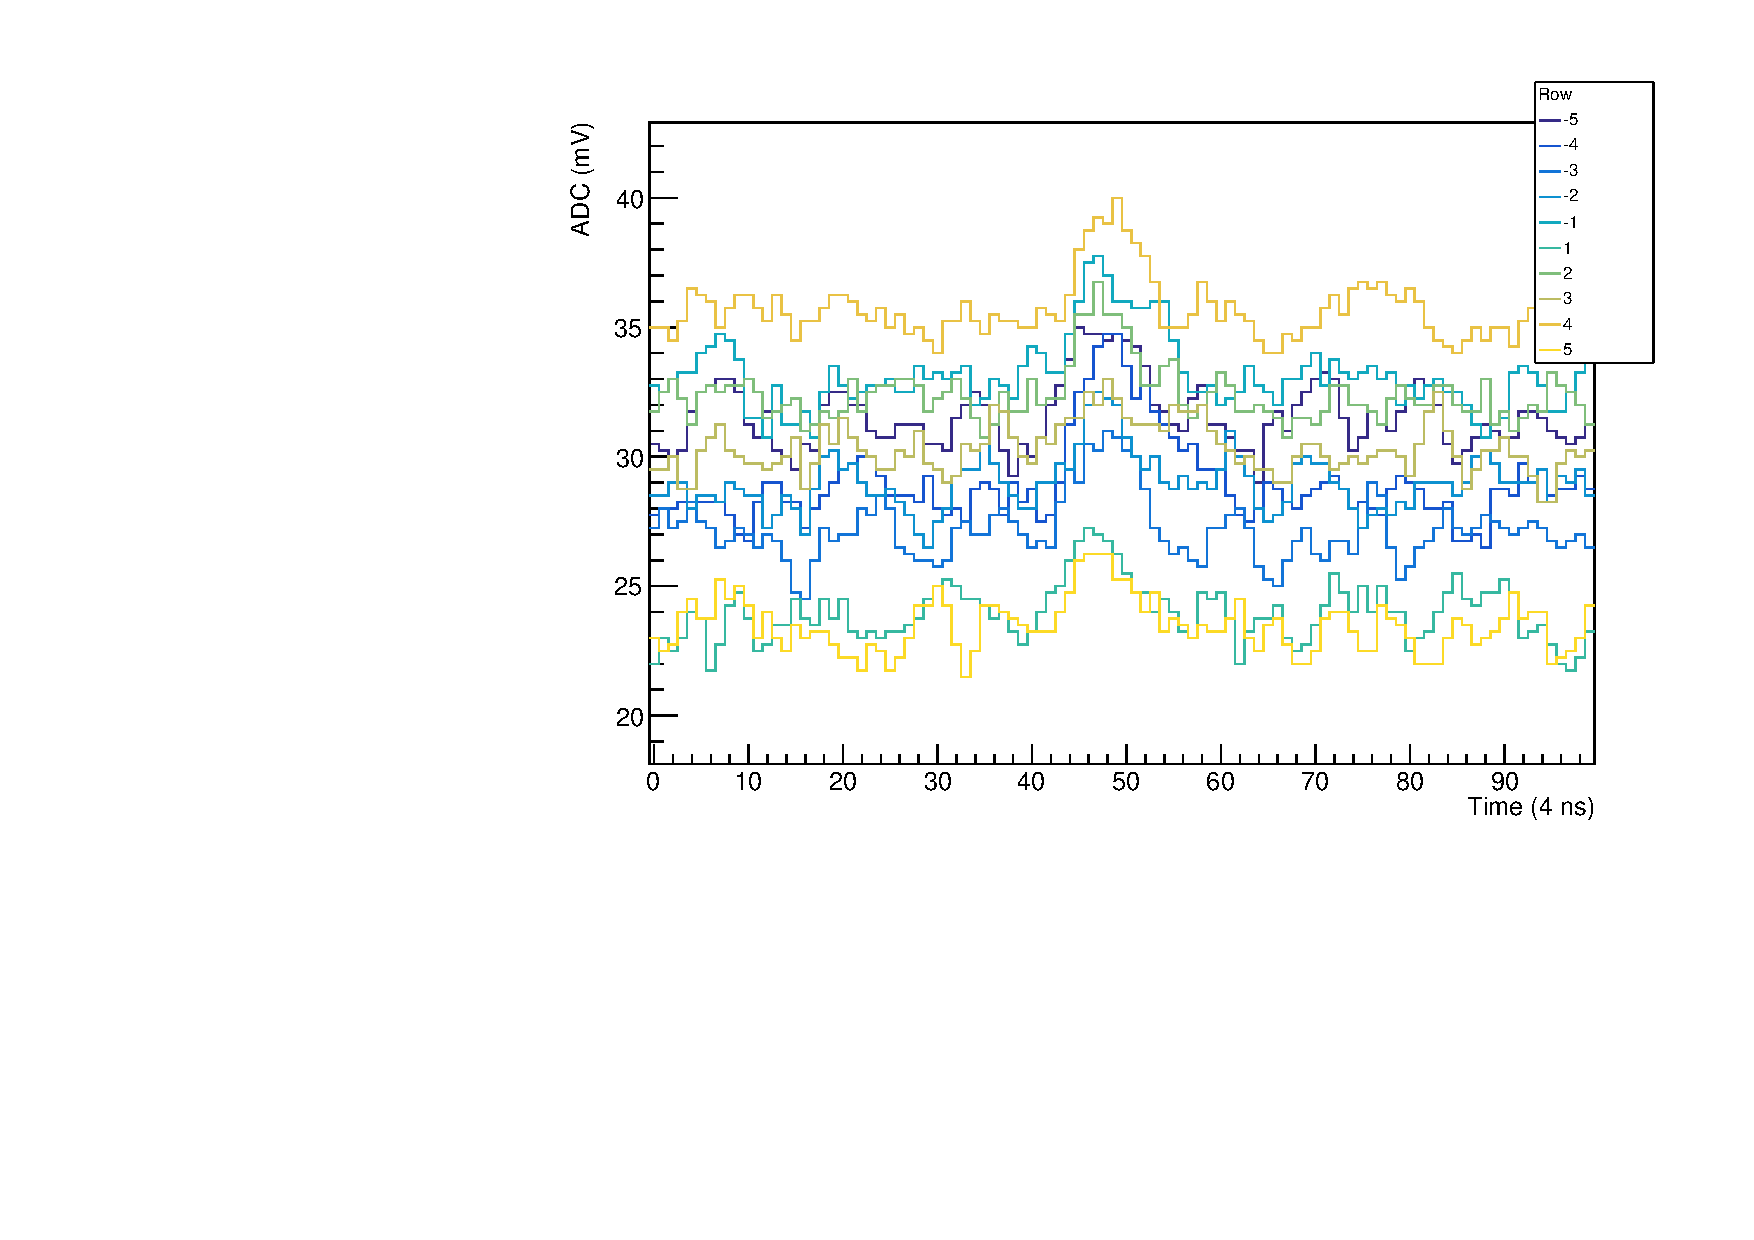
\includegraphics[width=0.8\textwidth]{pics/rayPassingVertically.pdf}
  \caption{Cosmic ray signal as seen when passing vertically through a column of ten crystals in the ECal.}
  \label{rawColumn}
\end{figure}	
In order to use the relatively small signals from cosmic rays in the ECal, cuts are applied to isolate the peak. The goal of the cuts is to ensure that the signal is from a cosmic ray muon (as opposed to a fluctuation in the FADC channel spectra) and that the hit passes cleanly through the crystal of interest such that the energy is not shared between crystals in the same row. From Figure~\ref{rawColumn}, it is clear that the signals are very close to the pedestal, but a threshold can be chosen from this raw spectrum to identify when a signal is visible in a crystal. With the splitters installed in the HPS detector setup, this threshold was 2.5~FADC mV. After removal of the splitters, the threshold was increased to XX~FADC mV. \\
\indent The threshold was used when applying geometric cuts to ensure that the cosmic ray muon passed vertically through the ECal. The geometric cuts were optimized from Monte Carlo to ensure that the signal is clearly visible in the crystal of interest. The analysis seeks crystals that have a threshold crossing in the optimal time window as prescribed from the DAQ. If there is a threshold crossing, then a threshold crossing is also required in the crystals immediately above and below the crystal of interest. A threshold crossing must not exist in the crystals to the immediate left and right of the crystal of interest in the same row. For edge crystals, the requirement to have a hit immediately above or below is altered such that the two subsequent crystals in the same column away from the edge have a hit above threshold.\\ 
\indent From previous work~\cite{charles_2014}, the ECal response is described by the sum of the pedestal and a {\em 3-pole} function:
\begin{equation}
  P\ +\ \frac{A}{2\tau^3}\ (t-t_0)^2\ e^{-(t-t_0)/\tau}
  \label{eqn:3pole}
\end{equation}
This function was further studied and implemented into the HPS calorimeter reconstruction software as described by~\cite{baltzell_ecal_2015}. Previously, the cosmic signals were integrated from the raw FADC spectra and not from a fit to the raw FADC spectra. Here, Equation~\eqref{eqn:3pole} is applied to the cosmic signals as shown in Figure~\ref{fig:rawFits}. The pedestals, $P$, for each fit are averaged over the bins at the front of the FADC timing window for each event. The widths, $\tau$, for each each fit are fixed from those previously found by~\cite{baltzell_ecal_2015}. The $t_0$ is initialized from the bin time at threshold crossing. The integral $A$ is initialized from XX.\\ 
\begin{figure}[H]
\begin{minipage}{0.5\textwidth}
 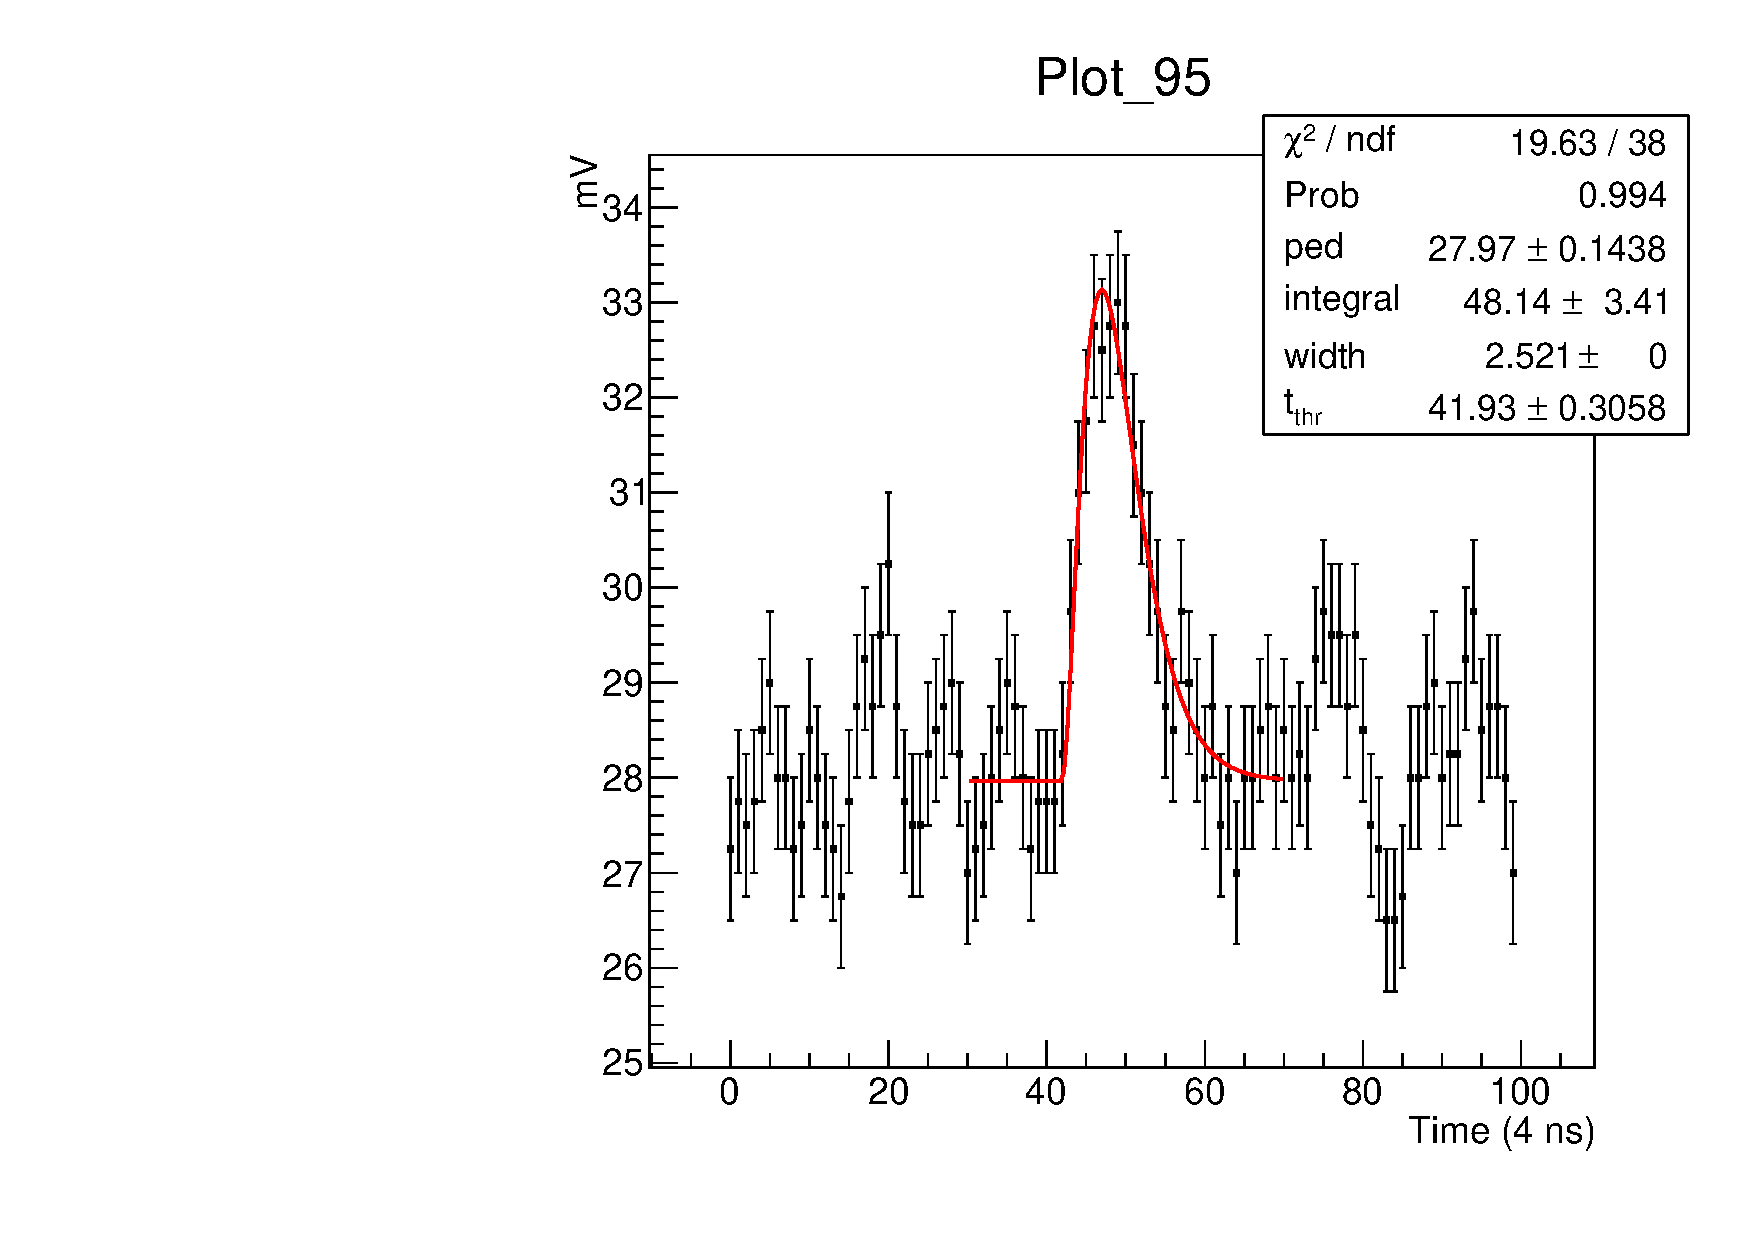
\includegraphics[width=\textwidth]{pics/rawfit2.pdf}
\end{minipage}\hfill\begin{minipage}{0.5\textwidth}
 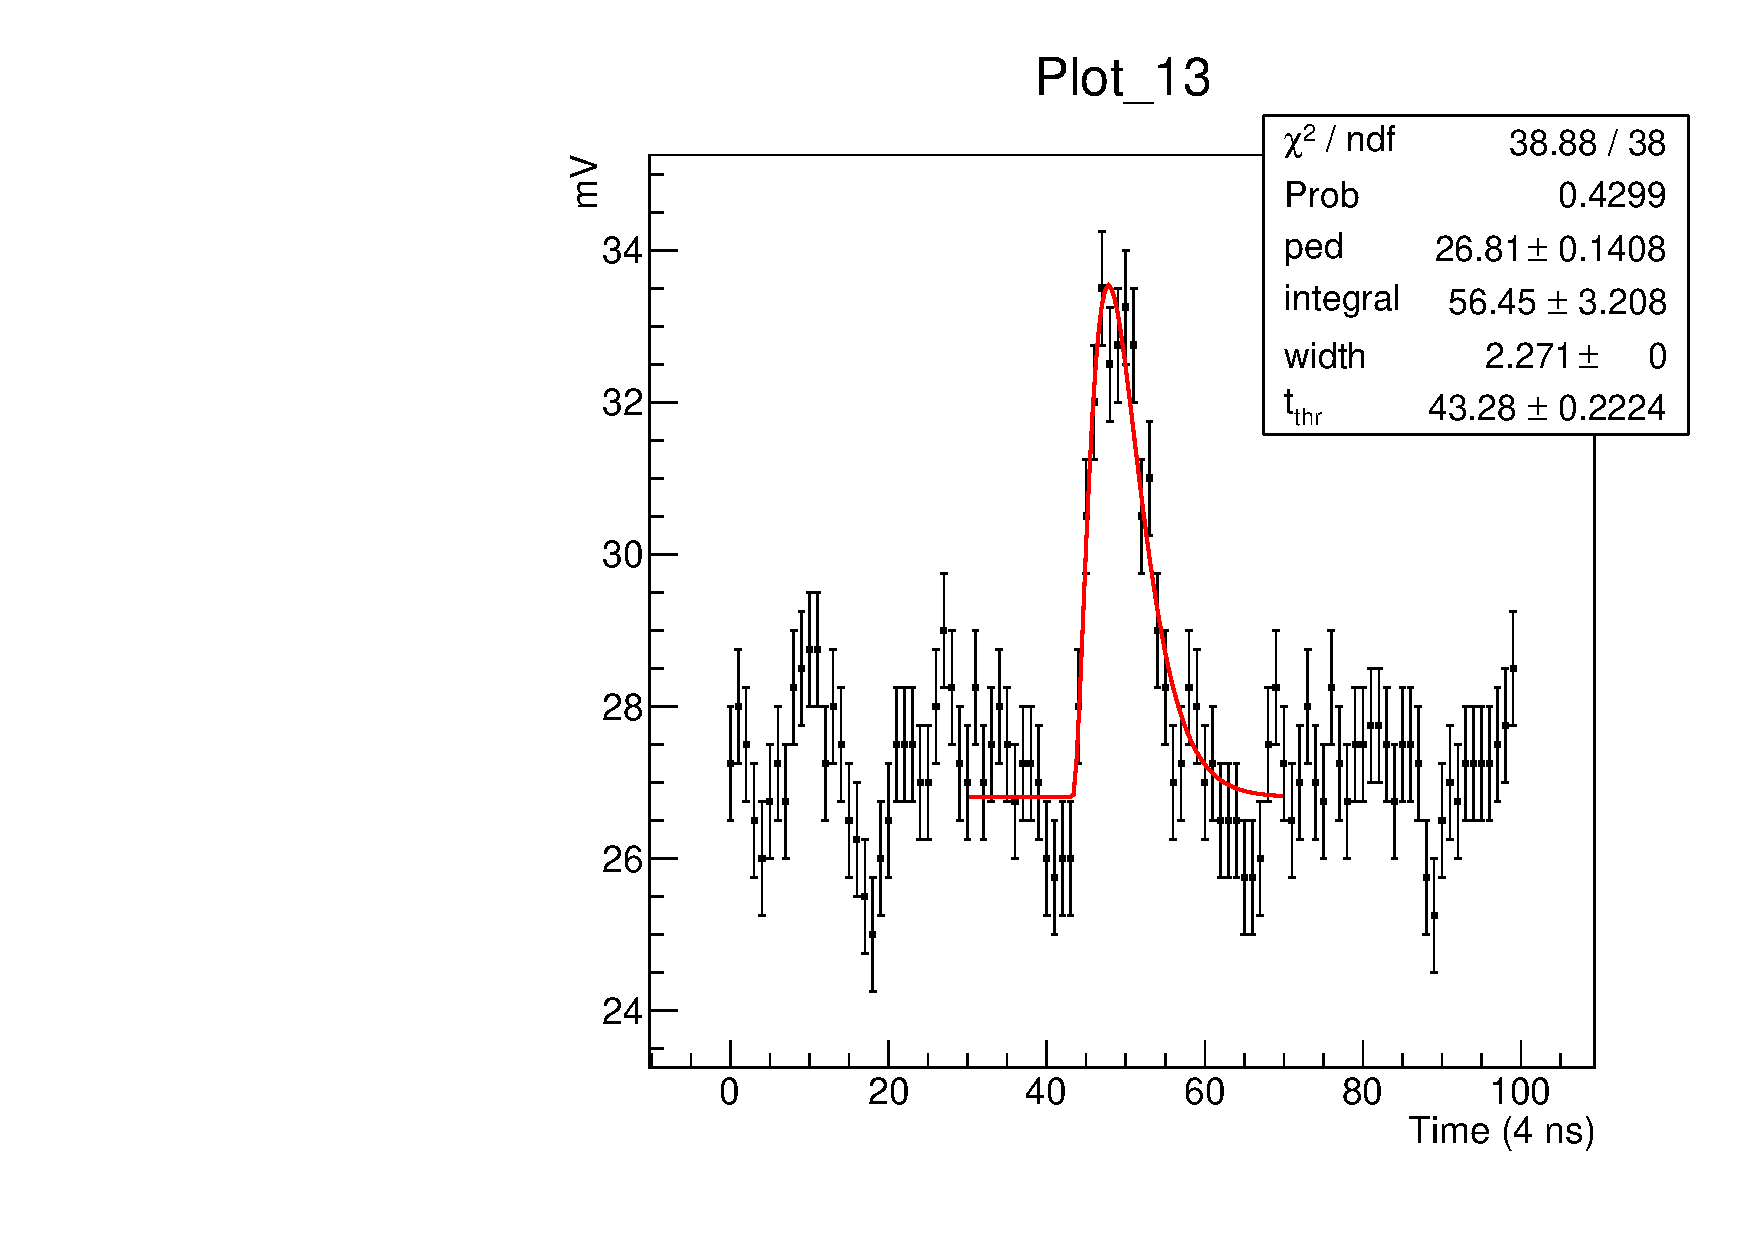
\includegraphics[width=\textwidth]{pics/rawfit3.pdf}
 \end{minipage}
 \begin{minipage}{0.5\textwidth}
  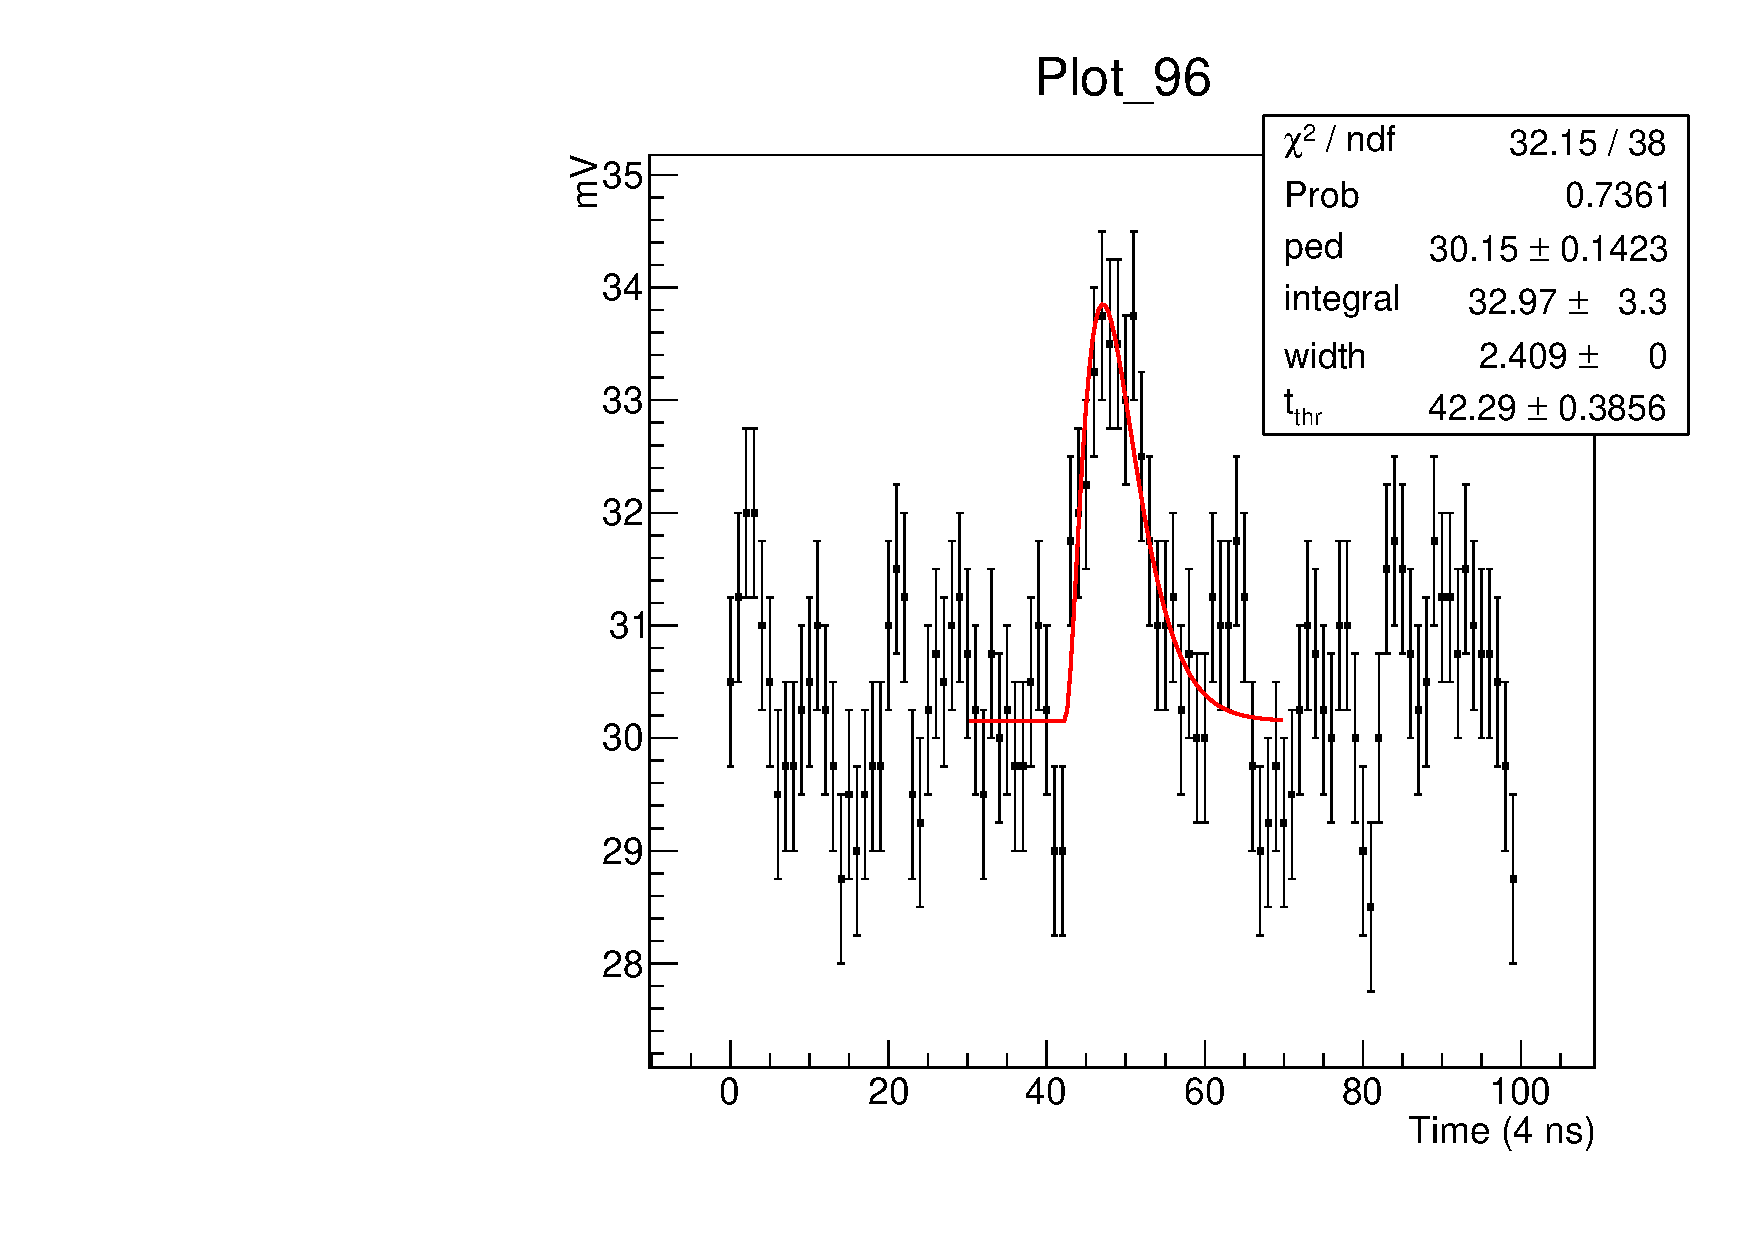
\includegraphics[width=\textwidth]{pics/rawfit1.pdf}
\end{minipage}\hfill\begin{minipage}{0.5\textwidth}
 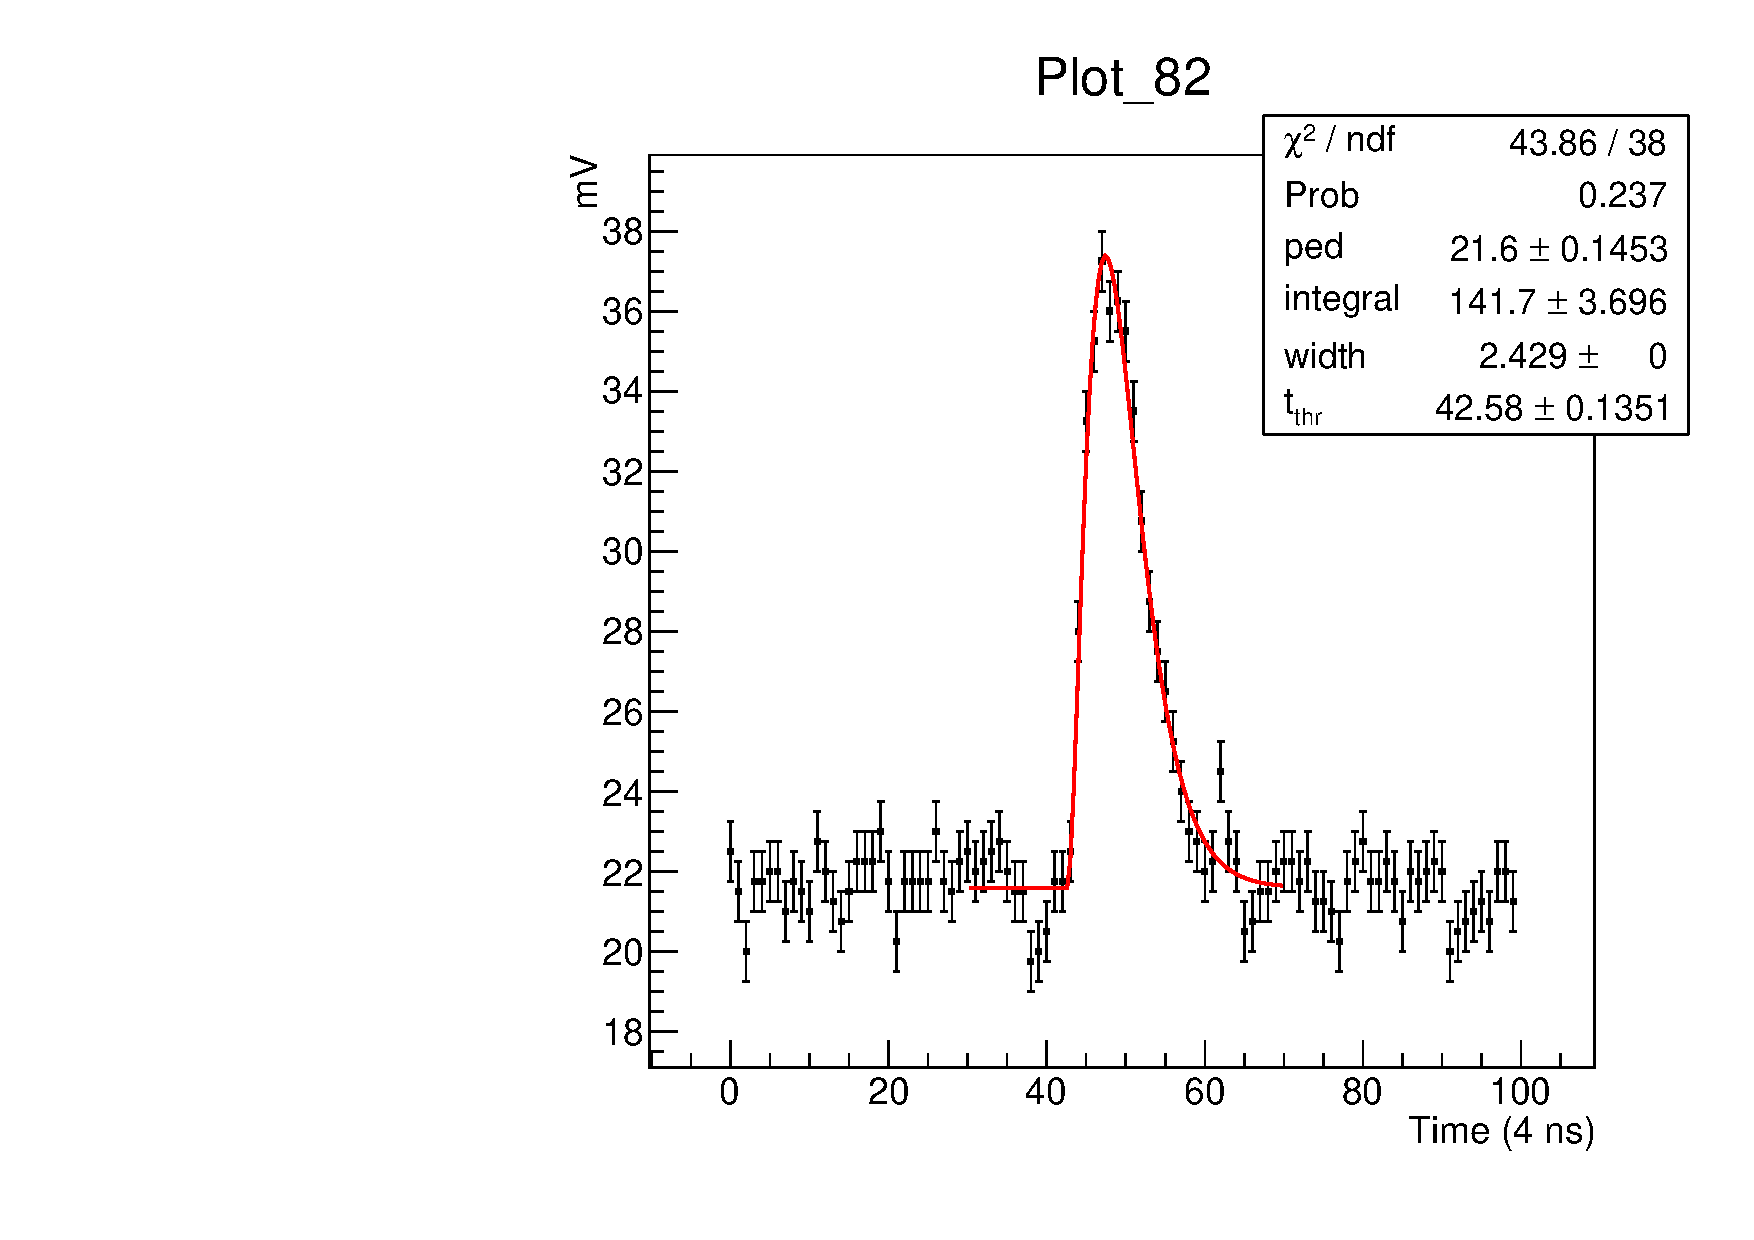
\includegraphics[width=\textwidth]{pics/rawfit4.pdf}
 \end{minipage}
  \caption{Fits applied to cosmic ray signals in four different crystals using Equation~\eqref{eqn:3pole}. The noise errors shown here are estimated to be XX~FADC mV per time bin.}
  \label{fig:rawFits}
\end{figure}
After applying the pulse-fitting procedure to the raw FADC spectra for each crystal, the peak position of the distribution of the pulse-integral per crystal is used to calibrate the gain. The pulse-integral distribution for a single crystal is shown in Figure~\ref{pulseIntFit}. The fit applied to Figure~\ref{pulseIntFit} is a Landau-Gaussian convolution where the Landau part arises from the scintillation response in the crystal, and the Gaussian component comes from the statistical noise component of the electronics in readout. 
\begin{figure}[htb]
  \centering
      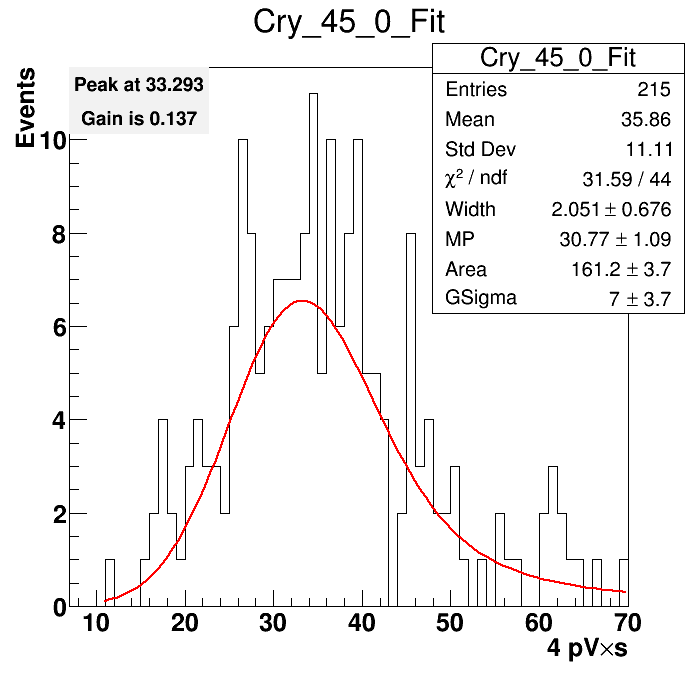
\includegraphics[width=0.5\textwidth]{pics/Cry_45_0_Fit.png}
  \caption{The pulse-integral distribution obtained from pulse-fitting applied to the raw FADC spectrum of each crystal is shown for a single crystal. The distribution is then fit with a Landau-Gaussian convolution, and the peak of this fit is obtained numerically to provide the calibration point.}
  \label{pulseIntFit}
\end{figure}	
The overall gain is obtained from numerically determining the peak position as shown in Figure~XXX and dividing into the expected energy deposition in the crystal as obtained from Monte Carlo. The formula is described by Equation~\eqref{eqn:gain}.
\begin{equation}
  \textrm{Gain} = \dfrac{\textrm{Energy }MeV}{\textrm{FADC pulse-integral}}
  \label{eqn:gain}
\end{equation}

%------------------------------------------------
\section{Results}
From the fits shown in Figure~\ref{fig:rawFits}, the $\chi^2$ distribution is shown in Figure~\ref{fig:chi2}. Here, the noise per bin is estimated to be XX~FADC mV. The resulting $\chi^2$ from these fits appears to be reasonable and is slightly worse than the quality described by~\cite{baltzell_ecal_2015}. The decrease in fit quality is most likely due to the low energy of the signals when compared to the signals in~\cite{baltzell_ecal_2015}.
\begin{figure}[hbt]
\begin{minipage}{0.5\textwidth}
 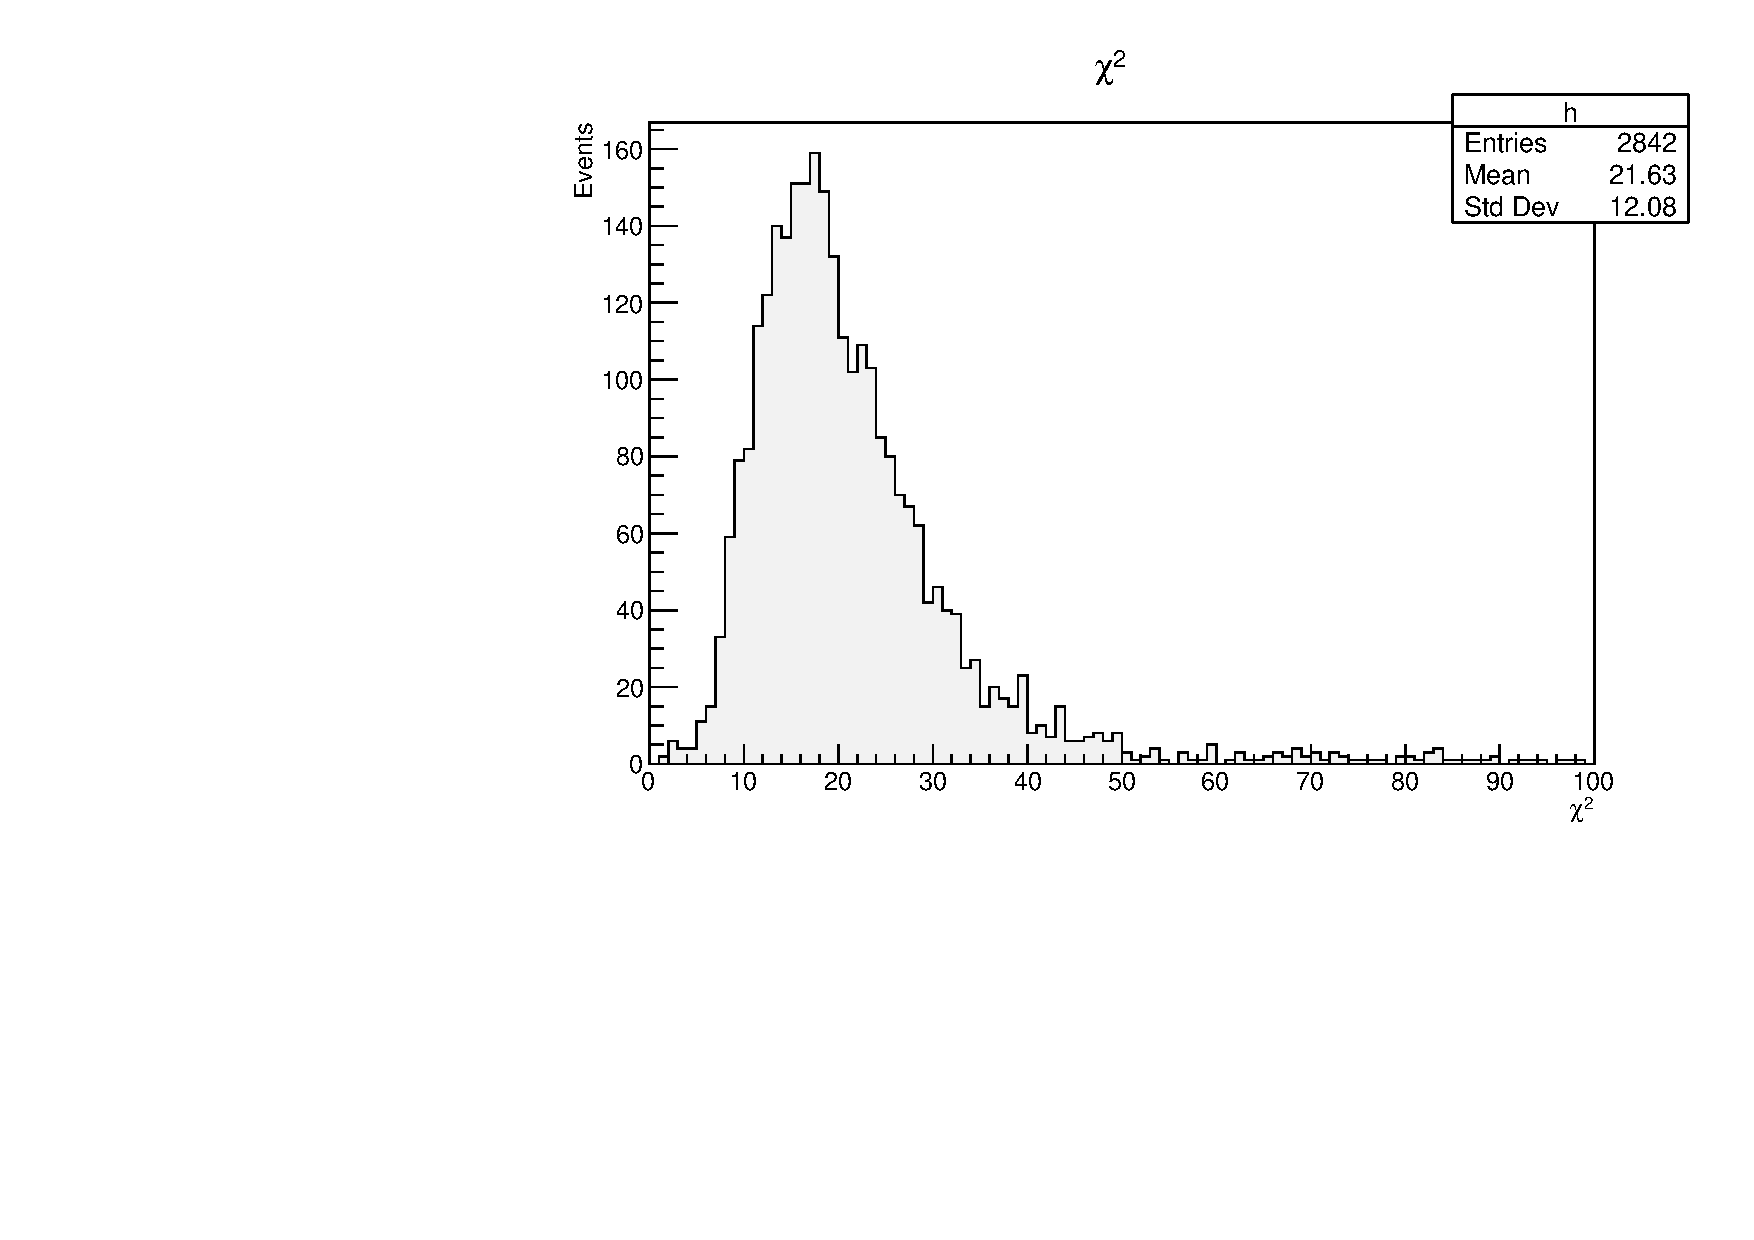
\includegraphics[width=\textwidth]{pics/chi2.pdf}
\end{minipage}\hfill\begin{minipage}{0.5\textwidth}
 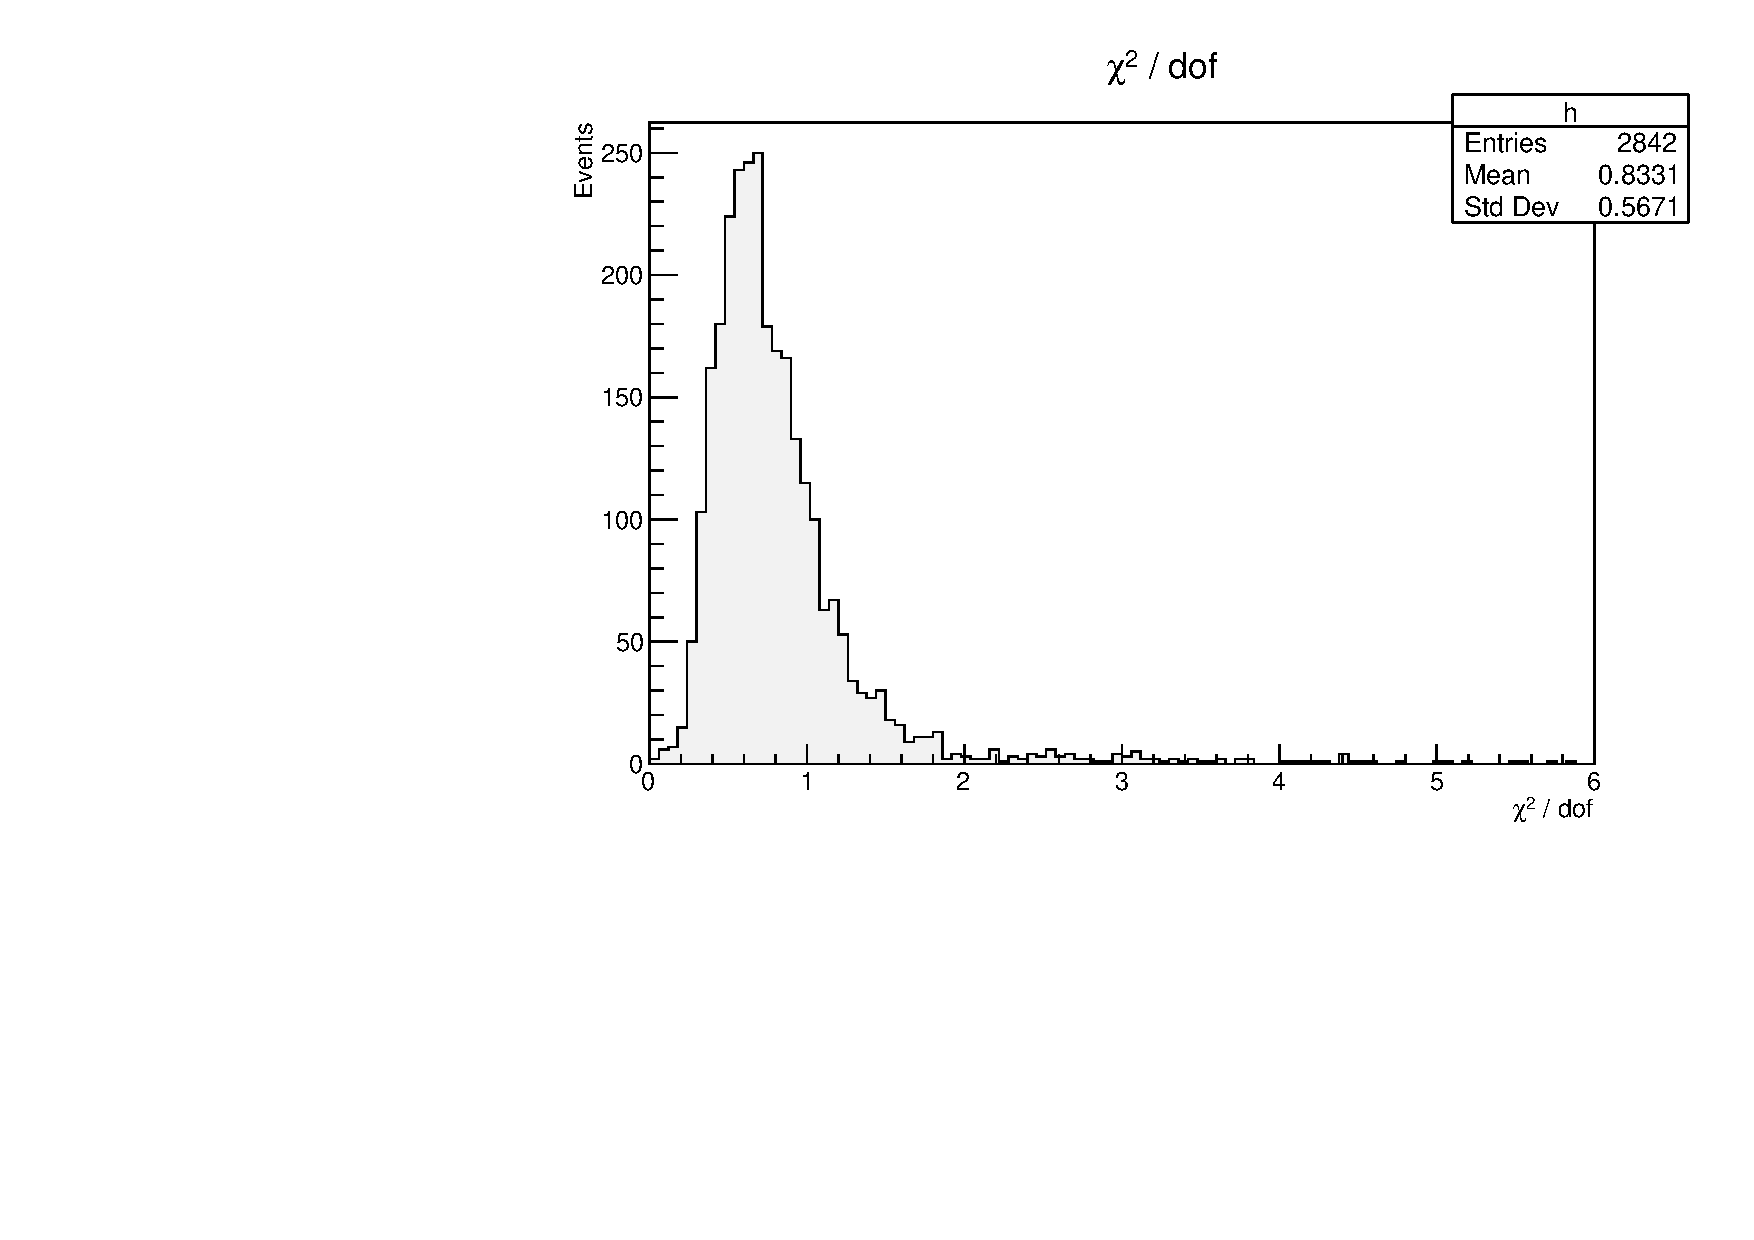
\includegraphics[width=\textwidth]{pics/chi2_dof.pdf}
 \end{minipage}
  \caption{Shown on the left is the raw $\chi^2$ distribution from the pulse-fits applied to cosmic ray signals in the ECal. The $\chi^2/dof$ is shown on the right. The distribution on the right looks reasonable, but is slightly worse than the distribution obtained~\cite{baltzell_ecal_2015} due to the low energy of the signals.}
  \label{fig:chi2}
\end{figure}
We compare the fits to the pulse-integral distributions to understand the differences when obtaining the pulse-integral from the integral of the fit to the raw FADC spectra versus the integration of the raw FADC spectra without fitting. As shown in Figure~\ref{compare} on the left, the resulting Gaussian widths are relatively unchanged for the overall ECal response. This is not a truly accurate metric for comparison because the Gaussian widths are also strongly affected by the Landau part of the fit and this is mainly responsible for the outliers. However, it can be seen that there is generally no overall systematic difference or improvement. The peak of the pulse-integral distribution from pulse-fitting is shifted to larger values as shown in Figure~\ref{fig:compare} on the right. This larger value probably results from the visible dips in the FADC spectra that can be seen in Figure~\ref{fig:rawFits}. These dips would not significantly affect the integral of the distribution when fitting as they would when integrating the raw FADC spectrum.
\begin{figure}[hbt]
\begin{minipage}{0.5\textwidth}
 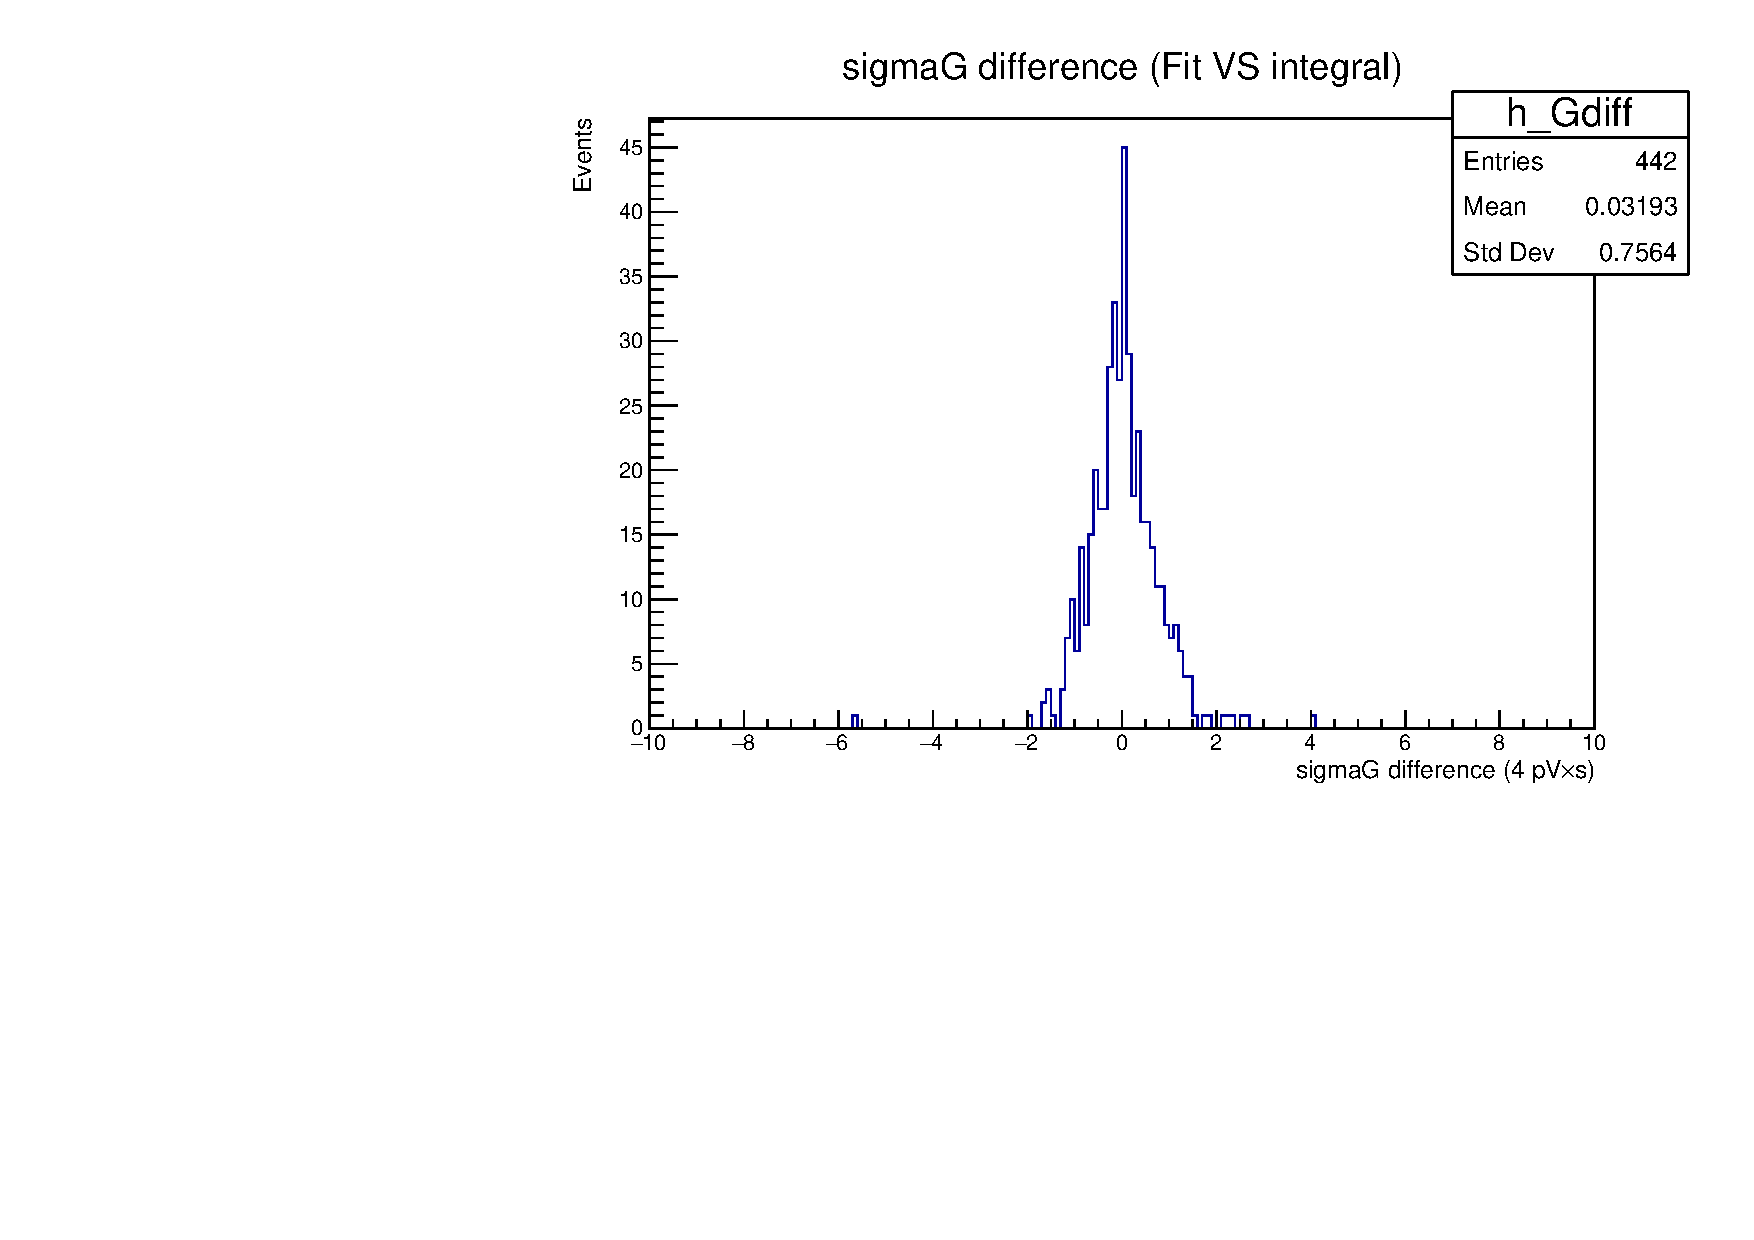
\includegraphics[width=\textwidth]{pics/cosmicGdiff.pdf}
\end{minipage}\hfill\begin{minipage}{0.5\textwidth}
 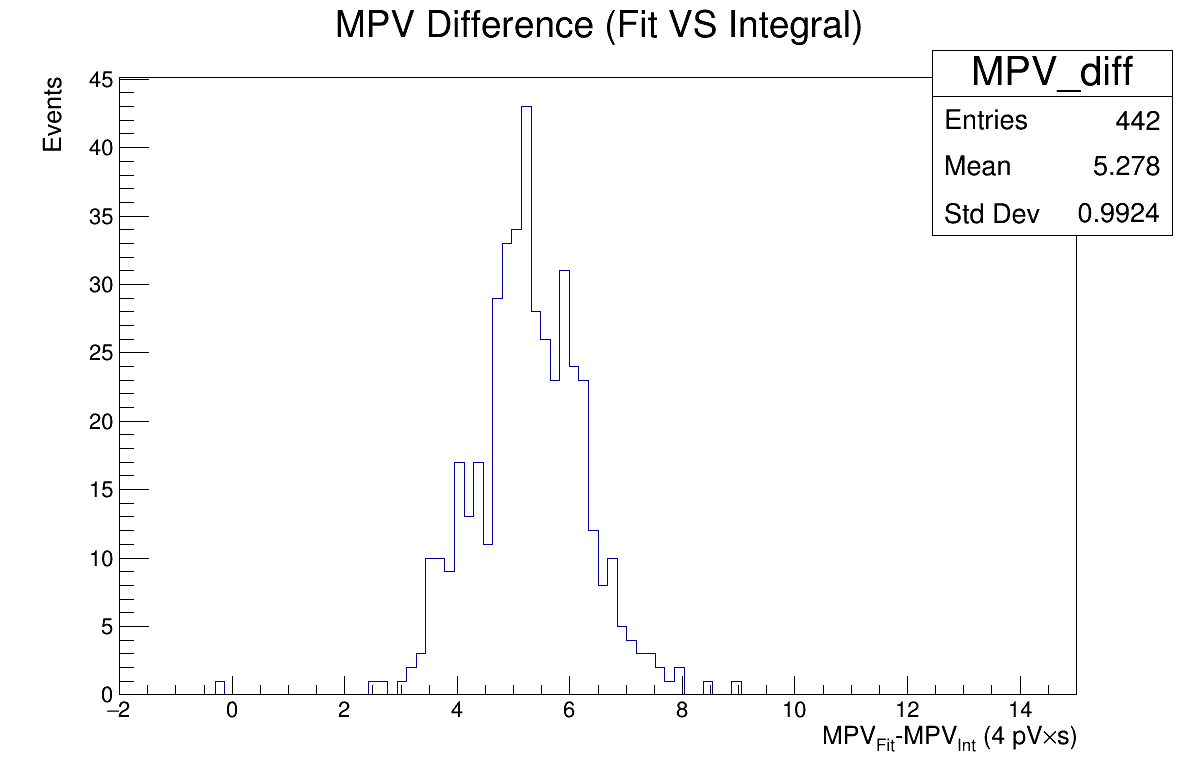
\includegraphics[width=\textwidth]{pics/cosmicMPVdiff.png}
 \end{minipage}
  \caption{A comparison of the Gaussian $\sigma$ from the convolution fit to the distribution of the pulse-integrals is compared for the pulse-integrals obtained from fitting and non-fitting procedures on the left. A comparison between the peak position from the distributions is shown on the right. While the resolution appears to be roughly the same, the peak position is systematically higher when the pulse-integral is obtained using pulse-fitting.}
  \label{fig:compare}
\end{figure}
While no clear improvement is achieved for the overall ECal using pulse-fitting, crystals that had relatively noisy distributions tended to produce much cleaner distributions with pulse-fitting. A more typical improvement is shown in Figure~\ref{fig:compareResults}.\\
%It would be good to find the Crystal 45,6 from earlier runs that had a more marked improvement. Maybe we can find a different crystal for this.
\begin{figure}[hbt]
\begin{minipage}{0.5\textwidth}
 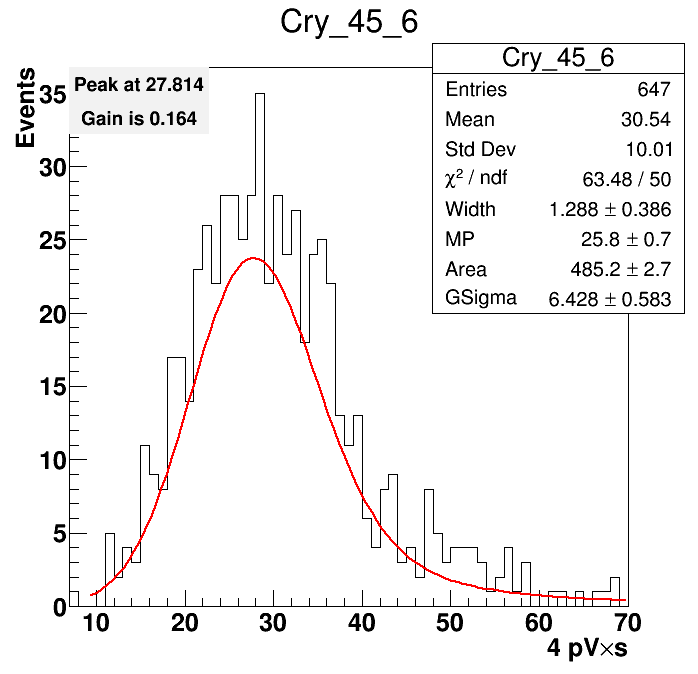
\includegraphics[width=\textwidth]{pics/Cry_45_6.png}
\end{minipage}\hfill\begin{minipage}{0.5\textwidth}
 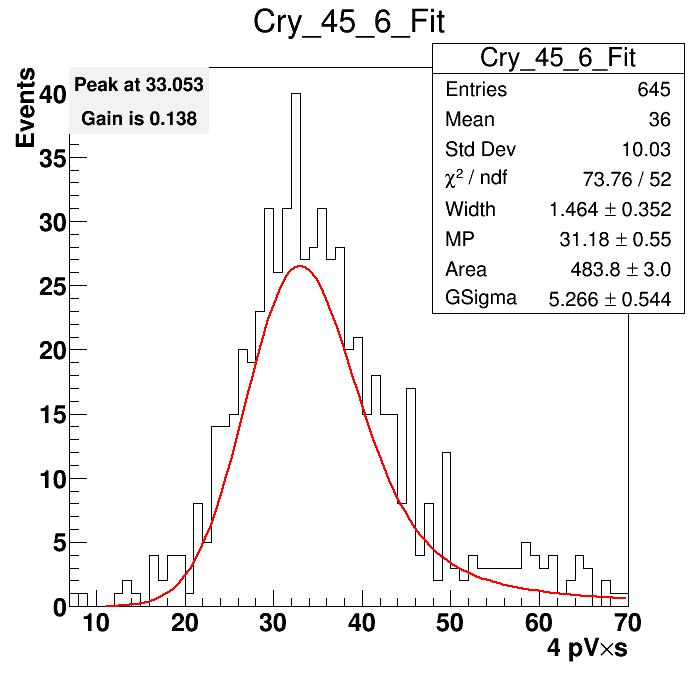
\includegraphics[width=\textwidth]{pics/Cry_45_6_Fit.png}
 \end{minipage}
  \caption{Shown on the left is the resulting pulse-integral distribution and fit for integration with no pulse-fitting. The right plot shows the resulting pulse-integral distribution for the same crystal whose pulse-integral was obtained with pulse-fitting.}
  \label{fig:compareResults}
\end{figure}
\indent From Monte Carlo simulation, the energy found to be deposited in the crystals using the prescribed geometric cuts was 16.7~MeV. After using this value for initial calibrations without pulse-fitting for the 2014 HPS run, the energy point was found to be too low when compared to the resulting peak position for elastically-scattered beam energy electrons. The energy for calibration point was increased to 18.3~MeV and appeared to provide a consistent calibration for all other energies as there was no longer a systematic offset with respect to the cosmic calibration. From this analysis, it is clear that pulse-fitting results in a systematically higher calibration point in cosmics. In order to establish gains that would be consistent with those seen from the elastically-scattered electron calibration from previous runs, the pulse-fitting cosmic calibration should using the previously found lower energy of 16.7~MeV for the gains. 

%If time, re-calibrate using elastically-scattered electrons and see if there is any improvement to the overally energy resolution

%------------------------------------------------
\section{Conclusion}
The selection criteria for choosing crystals with good cosmic events is the same as determined previously and still requires a significant time collecting signals. While the overall trigger rate for signals is apprixomately 7~Hz from the DAQ, the rates per crystal after all cuts are applied are XX~mHz. In order to accomplish a confident calibration of the ECal, it is necessary to run for at least XX~hours. A good calibration using the ECal is important in establishing preliminary gains for use in the DAQ and is critical to the calibration of crystals that are not within the acceptance for elastically-scattered beam energy electrons. No improvement to the time spent collecting cosmic signals is found using this method.\\
\indent The initialization of the fit parameters and the thresholds were thoroughly studied and discussed here. While pulse-fitting does not appear to improve the energy resolution of the ECal as a whole, there is improvement to some crystals that responded poorly when simply integrating the raw FADC spectrum. Pulse-fitting provides an improvement in the calibration of these crystals and is consistent with the HPS ECal reconstruction framework.\\

\section{Software packages}
The software is in the hps-java framework. Information for running the analysis can be found at https://github.com/JeffersonLab/HPS-CODE/tree/master/CALIBRATION/COSMIC.
%Can add in further description here of where the relevant steering file is in hps-java


%----------------------------------------------------------------------------------------
%	REFERENCE LIST
%----------------------------------------------------------------------------------------

\bibliography{biblio}{}
\bibliographystyle{unsrt}


%----------------------------------------------------------------------------------------
\end{document}